\documentclass[review]{elsarticle}
\usepackage{lineno}
\usepackage{amssymb}
\usepackage{amsmath}
\usepackage{booktabs}
\usepackage{longtable}
\usepackage{siunitx}
\usepackage{enumitem}
\usepackage{graphicx}
\usepackage{float}
\usepackage{placeins}
\usepackage{dblfloatfix}
\usepackage{xcolor}
\usepackage{hyperref}
\journal{Engineering Applications of Artificial Intelligence}
\date{}
\newcommand{\code}[1]{\path{#1}}
\newcommand{\benchfig}[2]{%
\IfFileExists{#1}{\includegraphics[width=\columnwidth]{#1}}{\fbox{\parbox{0.9\columnwidth}{#2\\\path{#1}}}}%
}
\makeatletter
\renewcommand{\topfraction}{0.85}
\renewcommand{\bottomfraction}{0.85}
\renewcommand{\textfraction}{0.15}
\renewcommand{\floatpagefraction}{0.90}
\renewcommand{\dbltopfraction}{0.85}
\renewcommand{\dblfloatpagefraction}{0.90}
\setcounter{topnumber}{2}
\setcounter{bottomnumber}{2}
\setcounter{totalnumber}{4}
\setcounter{dbltopnumber}{2}
\makeatother
\raggedbottom

\begin{document}
\linenumbers
\begin{frontmatter}
\title{Performance Benchmarking of Embedded Battery State Estimation: A Measurement-Only Comparison of Direct-Measurement, Hybrid, and Data-Driven Estimators}
\author[1]{[Author Placeholder]}
\affiliation[1]{organization={[Institution Placeholder]}, city={[City Placeholder]}, country={[Country Placeholder]}}
\begin{abstract}
This paper presents a measurement-only performance benchmark for embedded battery state estimation under realistic Battery Management System (BMS) constraints. Within the broader requirement space of embedded BMS algorithms, the study deliberately focuses on estimator performance rather than on hardware-resource or implementation-effort evaluation. Four embedded-ready estimators are compared on the same Lithium Iron Phosphate (LFP) full-cell trajectory as representative instances of four major estimator classes under a shared embedded hardware envelope: a direct-measurement model (DM), a hybrid direct-measurement model with learned State-of-Health support (HDM), a hybrid equivalent-circuit model with voltage feedback (HECM), and a data-driven neural model with GRU-based SOC estimation and LSTM-based online SOH context (DD). The benchmark perturbs only measurable inputs and timing information, including current bias, current noise, voltage noise, temperature noise, missing samples, irregular sampling, burst dropouts, spikes, and initial-state mismatch, so that all disturbances remain physically interpretable and reproducible without introducing artificial model-parameter mismatch. The resulting comparison reveals no universal winner across deployment-relevant performance dimensions. On the benchmark trajectory, HDM provides the best clean-condition baseline with an MAE of $0.0024$, followed by HECM with $0.0090$, DD with $0.0100$, and DM with $0.0311$, making HDM the accuracy leader. Under realistic current bias, HECM is clearly the most robust estimator, reaching an MAE of $0.0932$, compared with $0.2859$ for DD, $0.3068$ for HDM, and $0.3143$ for DM; together with its strong voltage-noise resilience, this makes HECM the overall robustness leader in the present benchmark. Under missing samples, DD remains particularly stable, changing only from $0.0100$ to $0.0117$ MAE, whereas the integration-based estimators degrade much more strongly. A local recovery analysis in a reset-free evaluation window further reveals a separate convergence ranking, with DD recovering fastest under both strict and fair criteria, HECM recovering more slowly, and HDM showing persistent mismatch in the inspected window. The benchmark therefore exposes complementary failure modes of direct-measurement, hybrid physics-based, and data-driven estimators and supports decision-oriented model selection for embedded BMS deployment.
\end{abstract}
\begin{keyword}
Battery management system \sep State of charge \sep State of health \sep Performance benchmark \sep Direct measurement \sep Equivalent circuit model \sep Data-driven estimation \sep Embedded artificial intelligence
\end{keyword}
\end{frontmatter}

\section*{Nomenclature}
\small
\subsection*{Acronyms}
\begin{description}[style=multiline,leftmargin=1.7cm,font=\bfseries]
\item[BMS] Battery management system
\item[SOC] State of charge
\item[SOH] State of health
\item[DM] Direct-measurement model
\item[HDM] Hybrid direct-measurement model
\item[HECM] Hybrid equivalent-circuit model
\item[DD] Data-driven neural model
\item[ECM] Equivalent circuit model
\item[EKF] Extended Kalman filter
\item[MAE] Mean absolute error
\item[RMSE] Root-mean-square error
\item[ADC] Analog-to-digital converter
\item[CV] Constant-voltage phase
\item[OCV] Open-circuit voltage
\item[GRU] Gated recurrent unit
\item[LSTM] Long short-term memory
\item[LFP] Lithium iron phosphate
\end{description}
\medskip
\subsection*{Symbols}
\begin{description}[style=multiline,leftmargin=1.7cm,font=\bfseries]
\item[$t$] Time
\item[$I(t)$] Current signal at time $t$
\item[$U(t)$] Voltage signal at time $t$
\item[$T(t)$] Temperature signal at time $t$
\item[$\widehat{\mathrm{SOC}}(t)$] Estimated state of charge at time $t$
\item[$\widehat{\mathrm{SOH}}(t)$] Estimated state of health at time $t$
\item[$\mathrm{SOC}_{\mathrm{ref}}(t)$] Reference SOC target at time $t$
\item[$\mathrm{SOH}_{\mathrm{ref}}(t)$] Reference SOH target at time $t$
\item[$\Delta I$] Current bias or offset
\item[$\Delta U$] Voltage bias or offset
\item[$\Delta T$] Temperature bias or offset
\item[$\sigma_I$] Standard deviation of injected current noise
\item[$\sigma_U$] Standard deviation of injected voltage noise
\item[$\sigma_T$] Standard deviation of injected temperature noise
\item[$Q_c$] Online cumulative charge state used by the SOC models
\item[$C_{\mathrm{nom}}$] Nominal capacity
\item[$C_{\mathrm{eff}}$] Effective capacity used inside the estimator
\item[$U_{\max}$] Upper voltage threshold used for full-charge detection
\item[$U_{\mathrm{tol}}$] Voltage tolerance used in the full-charge condition
\item[$U_{1},U_{2}$] Polarization voltages of the first and second RC branch
\item[$\Delta\mathrm{MAE}$] Error increase relative to baseline
\end{description}
\normalsize

\section{Introduction}
\subsection{Motivation and practical relevance}
\begin{itemize}[leftmargin=*]
    \item Reliable battery state estimation is a core BMS function because SOC and SOH determine safety margins, usable energy, operating limits, charge control, and degradation-aware system management in both mobile and stationary lithium-ion battery applications \cite{shrivastavaReviewTechnologicalAdvancement2023,guoSystematicReviewElectrochemical2024,yaoSmarterBatteryManagement2025b}.
    \item Practical deployment quality is not defined by clean-condition accuracy alone, because real BMS operation is exposed to sensor bias, additive noise, initialization uncertainty after restart, missing samples, irregular sampling, communication interruptions, and transient signal spikes caused by measurement-chain limitations or disturbances in the surrounding system \cite{liRobustnessSOCEstimation2015,naseriReliableWirelessBMS2025,bergerBenchmarkingBatteryManagement2024}.
    \item The relevant engineering question is therefore not only whether an estimator achieves low MAE under nominal measurements, but also whether it converges back to a reliable state after disturbed initialization and whether it remains stable under physically plausible measurement corruption.
    \item As summarized conceptually in Figure~\ref{fig:performance_requirements}, the present benchmark treats deployment-facing performance as a three-dimensional problem consisting of nominal accuracy, convergence behavior after state inconsistency, and robustness against disturbed measurements and signal-integrity faults, embedded within broader BMS requirements such as hardware constraints and implementation effort.
    \item The present study therefore does not claim to cover the full BMS requirement space; instead, it deliberately isolates the performance branch as the paper focus and uses it to compare representative estimator classes under identical measurement-side disturbances and a matched embedded-feasibility constraint.
    \item The benchmark reveals clear differences between estimator classes, showing that models with strong nominal accuracy do not necessarily provide the strongest disturbance performance and that representative direct-measurement, hybrid physics-based, and data-driven estimators respond differently to bias, missing samples, and re-initialization events.
\end{itemize}

\begin{figure*}[t]
    \centering
    \IfFileExists{figures/Schematics/BMS_Requirements.pdf}{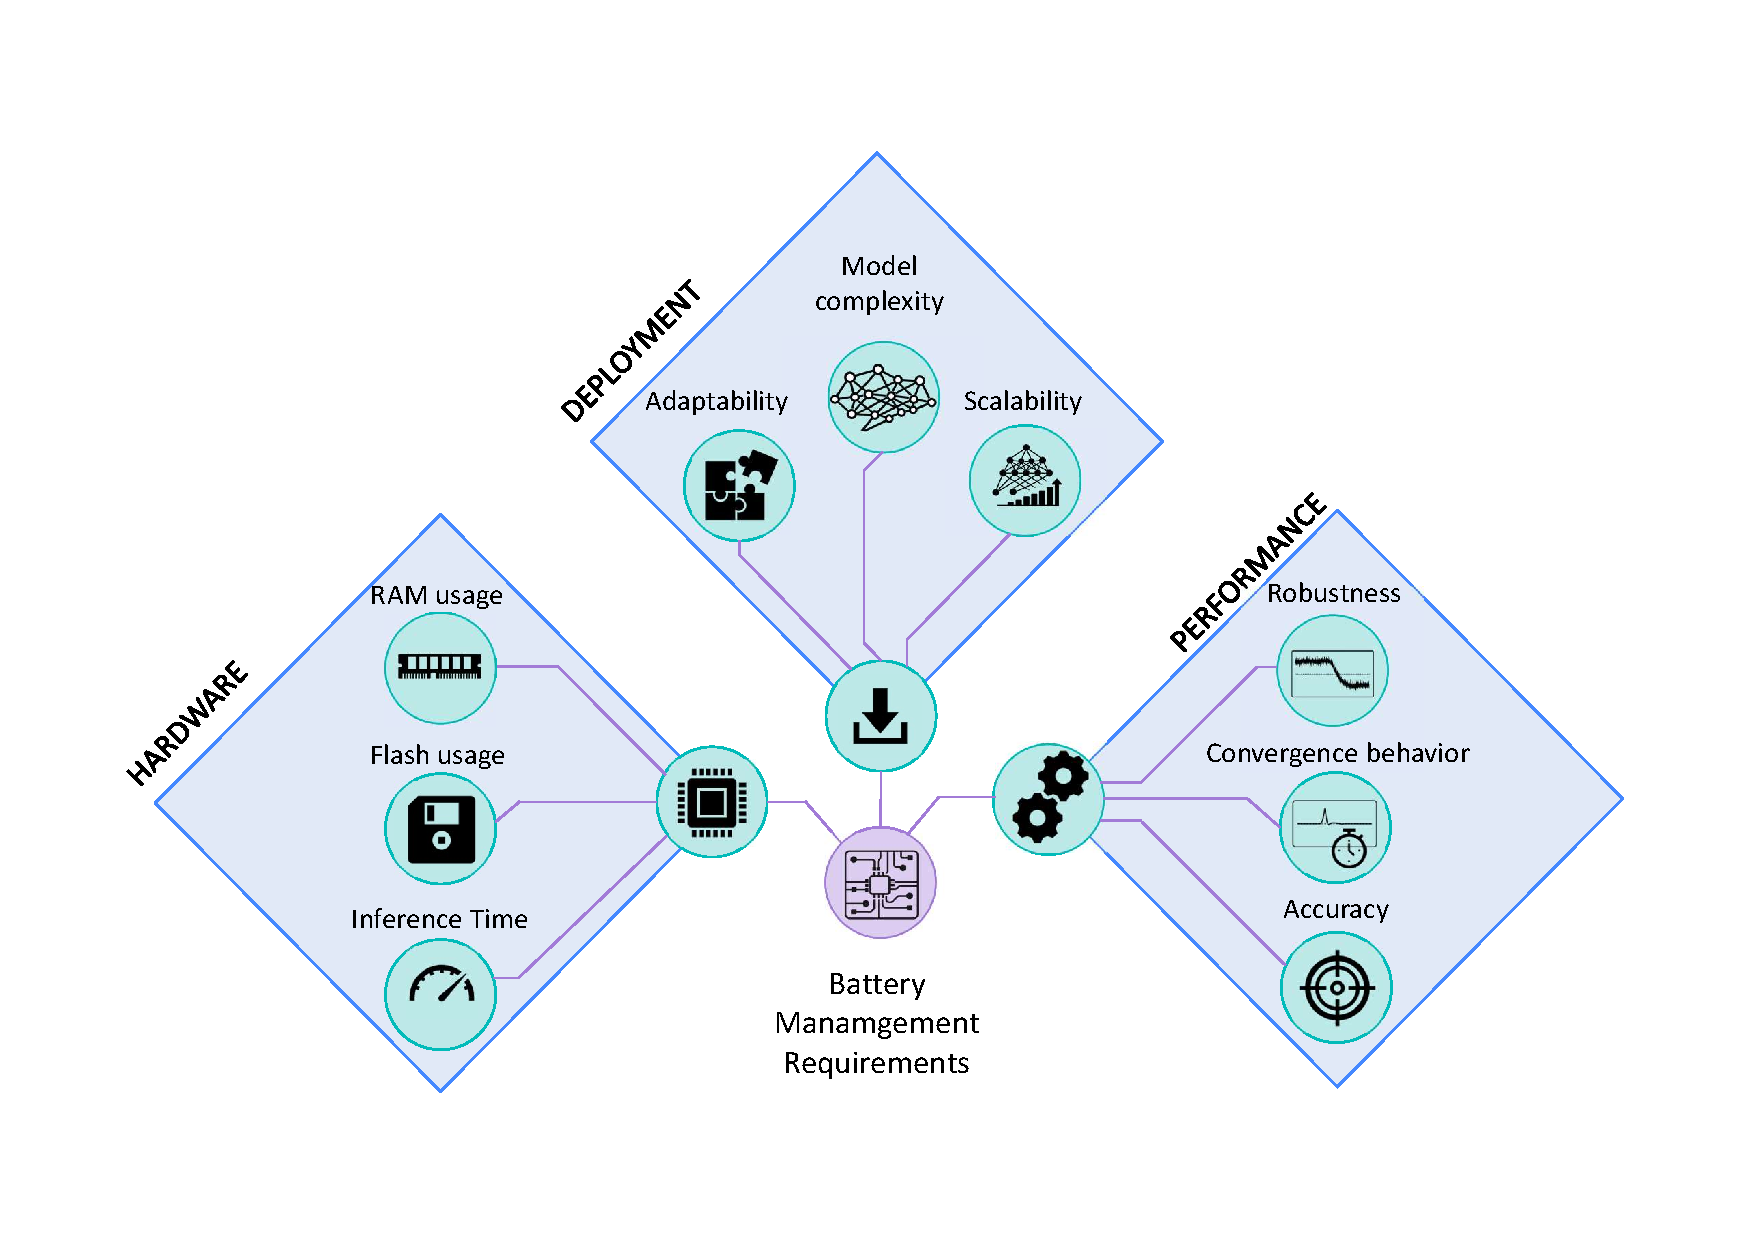
\includegraphics[width=0.98\textwidth,trim=12 12 12 12,clip]{figures/Schematics/BMS_Requirements.pdf}}{\fbox{\parbox{0.9\textwidth}{Placeholder for an adapted conceptual overview of deployment-oriented BMS state-estimation requirements. The figure should group requirements into implementation, hardware, and performance, and should explicitly highlight that the present study focuses on the performance branch with baseline accuracy, convergence behavior, and robustness.\\\path{figures/Schematics/BMS_Requirements.pdf}}}}
    \caption{Conceptual overview of deployment-oriented requirements for embedded BMS state estimation. The broader requirement space includes implementation effort, hardware constraints, and estimator performance, whereas the present study focuses on the performance branch and evaluates baseline accuracy, convergence behavior, and robustness under measurement disturbances.}
    \label{fig:performance_requirements}
\end{figure*}

\subsection{State of the art in battery state estimation}
\begin{itemize}[leftmargin=*]
    \item The literature commonly groups battery-state estimators into direct-measurement or integration-based approaches, model-based approaches based on equivalent-circuit or electrochemical models, hybrid approaches that combine physical structure with learned components, and purely data-driven models based on neural sequence learning \cite{khanComparativeStudyDifferent2022,shrivastavaReviewTechnologicalAdvancement2023,guoSystematicReviewElectrochemical2024,yaoSmarterBatteryManagement2025b}.
    \item Direct-measurement approaches, typically based on Coulomb counting, are attractive because they are simple, computationally inexpensive, and easy to deploy; however, they remain structurally sensitive to current bias, missing data, and initialization errors because they lack an internal correction mechanism \cite{khanComparativeStudyDifferent2022,liRobustnessSOCEstimation2015}.
    \item Model-based approaches, especially ECM- and observer-based estimators, offer physical interpretability and voltage-based correction capability. Their practical behavior nevertheless depends strongly on the quality of model parametrization, operating-point observability, and measurement quality \cite{gaoEnhancedStateofchargeEstimation2022,guoSystematicReviewElectrochemical2024,liRobustnessSOCEstimation2015}.
    \item Hybrid estimators seek to combine physical state propagation with learned adaptation of capacity, parameters, or auxiliary states, which has made joint SOC/SOH estimation an active research direction \cite{gaoCoEstimationStateofChargeStateof2022,shenAlternativeCombinedCoestimation2022,wangFusionEstimationLithiumion2022}. This combination can improve baseline calibration, while it does not necessarily eliminate structural sensitivity to measurement disturbances.
    \item Data-driven approaches based on recurrent or sequence models can exploit nonlinear cross-relations between current, voltage, temperature, and derived online features, and recent work has also demonstrated their embedded feasibility through TinyML-oriented implementations, pruning, and quantization \cite{mondalEstimatingStateofChargeLithiumIon2024,Embedded_AI_only_SOC_mobile,giazitzisCaseStudyTiny2024,mazziStateChargeEstimation2022,yaoSmarterBatteryManagement2025b}.
\end{itemize}

\subsection{Performance and embedded deployment gap}
\begin{itemize}[leftmargin=*]
    \item A large share of the SOC estimation literature still emphasizes clean-data accuracy, average error metrics, or computational efficiency, while comparatively fewer studies analyze how estimators behave under realistic measurement faults and timing corruption \cite{shrivastavaReviewTechnologicalAdvancement2023,Embedded_AI_only_SOC_mobile,giazitzisCaseStudyTiny2024,mazziStateChargeEstimation2022}.
    \item Existing robustness studies often remain confined to a single model family, for example observer-based robustness against modeling and measurement errors \cite{liRobustnessSOCEstimation2015} or robust estimation concepts for specific BMS architectures under noise and uncertainty \cite{naseriReliableWirelessBMS2025}, whereas cross-family comparisons under the same disturbance protocol and under comparable embedded constraints remain limited.
    \item Benchmarking studies in the broader BMS context underline the importance of reproducible scenario design and deployment-relevant validation, but they do not by themselves close the gap between clean-data estimator comparison and measurement-level performance benchmarking across fundamentally different estimator classes \cite{bergerBenchmarkingBatteryManagement2024}.
    \item This limitation becomes critical when estimator behavior must be evaluated under controlled, reproducible disturbances that reflect real measurement-chain imperfections.
    \item The embedded context further sharpens this gap, because estimator selection in a real BMS must simultaneously consider accuracy, convergence, robustness, and computational constraints under disturbed measurements together with nominal prediction quality.
\end{itemize}

\subsection{Contribution and study objectives}
\begin{itemize}[leftmargin=*]
    \item This work defines deployment-facing estimator performance as the joint assessment of nominal accuracy, convergence behavior after state inconsistency, and robustness under realistic disturbances applied only to measurable inputs and their timing.
    \item Within this performance framing, robustness denotes bounded global error increase, stable local behavior, limited drift, and recoverability after disturbance exposure.
    \item The study compares four representative estimator classes, namely a direct-measurement model (DM), a hybrid direct-measurement model with learned SOH support (HDM), a hybrid equivalent-circuit model with voltage feedback (HECM), and a data-driven neural model with stateful GRU-based SOC estimation and stateful LSTM-based online SOH context (DD), under identical online execution conditions.
    \item These implementations are interpreted as embedded-ready representatives of four major estimator families so that the comparison yields class-level insight in addition to model-specific results.
    \item The disturbances are deliberately restricted to measurement-level and signal-integrity scenarios, including current bias, current noise, voltage noise, temperature noise, missing samples, irregular sampling, burst dropouts, voltage spikes, and initialization errors, so that the benchmark remains physically interpretable and experimentally reproducible.
    \item The study objective is not only to compare average error values, but to identify which estimator class leads each deployment-relevant performance dimension, namely baseline accuracy, convergence after state inconsistency, and robustness under disturbed measurements.
    \item The manuscript should therefore be read as a controlled cross-class estimator benchmark and not as a complete system-level BMS validation campaign. Its contribution is to isolate estimator-side failure modes under matched data, matched disturbance definitions, matched online execution rules, and matched embedded-feasibility constraints.
    \item The core contribution is therefore a measurement-only performance benchmark that separates baseline accuracy from convergence behavior and disturbance robustness, and then translates the observed failure modes into deployment-oriented guidance for estimator selection in embedded BMS applications.
\end{itemize}

\section{Methodology}
\subsection{Estimator classes under test}
\begin{itemize}[leftmargin=*]
    \item The four selected implementations are treated as representative exemplars of broader estimator families, which means that the discussion focuses on structural class behavior and deployment implications of the estimator classes.
    \item The direct-measurement model (DM) represents the canonical embedded Coulomb-counting approach with fixed nominal capacity and explicit full-charge reset logic, and serves as the low-complexity reference for integration-driven SOC estimation.
    \item The hybrid direct-measurement model (HDM) preserves the same Coulomb-counting core but replaces the fixed capacity assumption with an online effective capacity derived from a learned SOH estimator, which makes it representative of lightweight hybrid estimation.
    \item The hybrid equivalent-circuit model (HECM) represents physics-based state estimation with observer correction, because it combines current-driven state propagation with voltage-residual feedback and SOH-dependent parameterization in a second-order RC equivalent-circuit structure \cite{gaoEnhancedStateofchargeEstimation2022,guoSystematicReviewElectrochemical2024}.
    \item The data-driven model (DD) represents a neural estimator pipeline in which SOC is predicted by a lightweight stateful GRU-based sequence model while online SOH context is provided by a separate stateful LSTM-based SOH estimator under the same causal execution constraints \cite{mondalEstimatingStateofChargeLithiumIon2024,yaoSmarterBatteryManagement2025b}.
\end{itemize}

\begin{figure*}[t]
    \centering
    \benchfig{figures/Schematics/methodology_overview.pdf}{Placeholder for a methodology overview figure showing the causal benchmark chain: measured current, voltage, temperature, and time signals; online reconstruction of auxiliary features such as $Q_c$, derivatives, EFC, and SOH context; execution of the four estimator classes; injection of measurement-only disturbance scenarios; and final global/local performance evaluation.}
    \caption{Methodology overview for the causal benchmark chain. Measured battery signals are converted into online auxiliary features, processed by representative estimator classes, exposed to measurement-only disturbances, and finally evaluated through global and local performance metrics.}
    \label{fig:methodology_overview}
\end{figure*}

\subsection{SOC estimation methods}
\subsubsection{Direct-measurement model (DM)}
\begin{itemize}[leftmargin=*]
    \item The direct-measurement SOC formulation used in DM, HDM, and as an explicit auxiliary feature in DD follows the same online cumulative-charge state, denoted here uniformly as $Q_c$. It is updated causally from the measured current stream as
    \begin{equation}
        Q_c(k)=Q_c(k-1)+\frac{I_k \Delta t_k}{3600\,\mathrm{s\,h^{-1}}},
        \label{eq:qc_update}
    \end{equation}
    where $I_k$ is given in ampere and $\Delta t_k$ in seconds, so that the factor $3600\,\mathrm{s\,h^{-1}}$ converts the increment to ampere-hours. The sign convention is fixed by the benchmark implementation and the state is reset to $Q_c=0$ after a sustained constant-voltage full-charge event. In the DM, this same charge state is mapped directly to SOC through the fixed nominal capacity
    \begin{equation}
        \widehat{\mathrm{SOC}}_{\mathrm{DM}}(k)=\mathrm{clip}\!\left(1+\frac{Q_c(k)}{C_{\mathrm{nom}}},0,1\right),
        \label{eq:soc_dm}
    \end{equation}
\end{itemize}

\subsubsection{Hybrid direct-measurement model (HDM)}
\begin{itemize}[leftmargin=*]
    \item The HDM preserves exactly the same Coulomb-counting core and differs only in the capacity term. The SOH estimate rescales the usable capacity as
    \begin{equation}
        C_{\mathrm{eff}}(k)=C_{\mathrm{nom}} \cdot \widehat{\mathrm{SOH}}(k),
        \label{eq:ceff}
    \end{equation}
    which yields
    \begin{equation}
        \widehat{\mathrm{SOC}}_{\mathrm{HDM}}(k)=\mathrm{clip}\!\left(1+\frac{Q_c(k)}{C_{\mathrm{eff}}(k)},0,1\right).
        \label{eq:soc_hdm}
    \end{equation}
    This formulation makes the relation between DM and HDM explicit: both use the same online charge state $Q_c$, while only the denominator changes through online SOH support.
    \item In both direct-measurement variants, a sustained near-maximum voltage condition is interpreted as a constant-voltage full-charge event; if the voltage remains above $U_{\max}-U_{\mathrm{tol}}$, where $U_{\mathrm{tol}}$ denotes the admissible voltage margin below the upper threshold $U_{\max}$, for the configured CV duration, the internal charge state is reset so that $Q_c=0$ and therefore $\widehat{\mathrm{SOC}}=1$, which reflects the practical assumption that a completed CV phase provides a physically anchored full-charge reference.
\end{itemize}

\subsubsection{Hybrid equivalent-circuit model (HECM)}
\begin{itemize}[leftmargin=*]
    \item The hybrid ECM model is implemented as a second-order RC model with the state vector
    \begin{equation}
        \mathbf{x}_k = \begin{bmatrix}\widehat{\mathrm{SOC}}_k & U_{1,k} & U_{2,k}\end{bmatrix}^{\top},
        \label{eq:ecm_state}
    \end{equation}
    where $U_1$ and $U_2$ denote the polarization voltages of the two RC branches. The prediction step propagates the state according to
    \begin{equation}
        \mathbf{x}_{k}^{-}=\mathbf{A}_k \mathbf{x}_{k-1}+\mathbf{b}_k I_{k-1},
        \label{eq:ecm_prediction}
    \end{equation}
    with
    \begin{equation}
        \mathbf{A}_k=\mathrm{diag}\!\left(1,e^{-\Delta t_k/\tau_1},e^{-\Delta t_k/\tau_2}\right),
        \quad
        \mathbf{b}_k=
        \begin{bmatrix}
            \eta \Delta t_k / C_b \\
            R_1\!\left(1-e^{-\Delta t_k/\tau_1}\right) \\
            R_2\!\left(1-e^{-\Delta t_k/\tau_2}\right)
        \end{bmatrix},
        \label{eq:ecm_ab}
    \end{equation}
    where $C_b=C_0 \widehat{\mathrm{SOH}}$ is the SOH-scaled available capacity. The corrected terminal-voltage estimate is written as
    \begin{equation}
        \widehat{U}_k = \mathrm{OCV}(\widehat{\mathrm{SOC}}_k,\widehat{\mathrm{SOH}}_k,I_k) + U_{1,k} + U_{2,k} + R_i I_k,
        \label{eq:ecm_voltage}
    \end{equation}
    and the Kalman update uses the residual between $\widehat{U}_k$ and the measured terminal voltage to correct the internal state. In the present implementation, the state propagation is driven by the previous current sample $I_{k-1}$, whereas the measurement equation uses the current sample $I_k$ available at the correction step.
    \item The ECM parameters are not constant. The implementation interpolates $R_i$, $R_1$, $R_2$, $\tau_1$, $\tau_2$, $\mathrm{OCV}$, and $\mathrm{dOCV}/\mathrm{dSOC}$ from a preidentified lookup table over SOC and SOH, with separate charge and discharge parameter surfaces. The HECM is implemented as a two-RC observer with SOH-dependent parameter scheduling.
\end{itemize}

\subsubsection{Data-driven SOC model (DD)}
\begin{itemize}[leftmargin=*]
    \item The data-driven SOC model is a stateful GRU-based recurrent estimator with the feature vector \{$U$~[V], $I$~[A], $T$~[$^\circ$C], SOH, $Q_c$, $dU/dt$, $dI/dt$, $\Delta t$\}. The network consists of a single-layer GRU with hidden size $96$ followed by an MLP head with one hidden layer of size $96$ and a sigmoid output layer. During optimization, the recurrent core is exposed to causal sequence segments of length
    \begin{equation}
        L_{\mathrm{SOC}} = 2024
    \end{equation}
    samples.
    \item Within this feature set, $Q_c$ is exactly the same online cumulative-charge state defined in \eqref{eq:qc_update}. It is included explicitly so that the neural estimator receives the same charge-throughput information that also drives DM and HDM.
    \item The derivative channels are computed online as finite differences with respect to the current sampling interval,
    \begin{equation}
        \frac{\mathrm{d}I}{\mathrm{d}t}(k)=\frac{I_k-I_{k-1}}{\Delta t_k},
        \qquad
        \frac{\mathrm{d}U}{\mathrm{d}t}(k)=\frac{U_k-U_{k-1}}{\Delta t_k},
        \label{eq:derivative_features}
    \end{equation}
    and provide the neural estimator with local transient information on current and voltage dynamics that is not directly captured by the absolute channel values alone. The additional feature $\Delta t_k$ is passed explicitly so that the network can distinguish amplitude changes from sampling-interval changes under irregular timing.
    \item During benchmark execution, the GRU is used as a causal stateful estimator with persistent hidden-state forwarding. No future information is used, and the MLP head is applied at every recurrent step so that a continuous SOC trajectory is obtained directly from the evolving recurrent state.
    \item This execution scheme is consistent with BMS-oriented embedded deployment, because the SOC network is used as a recurrent estimator with persistent memory along the causal measurement stream.
\end{itemize}

\subsection{SOH estimation method}
\begin{itemize}[leftmargin=*]
    \item The shared SOH estimator used in the current benchmark is an LSTM-based sequence-to-sequence model that operates on hourly aggregated online features derived from \{$U$~[V], $I$~[A], $T$~[$^\circ$C], EFC, $Q_c$\}, where the aggregation uses the statistics mean, standard deviation, minimum, and maximum for each feature \cite{Embedded_AI_SOH_badData,gouEnsembleLearningBasedDataDriven2021,liOnlineCapacityEstimation2021,rzepkaNeuralNetworkArchitecture2023a}. This transforms the five base channels into a $20$-dimensional hourly feature vector.
    \item Architecturally, the SOH network first projects the aggregated input through a two-layer feature embedding block with size $128$, layer normalization, GELU activations, and dropout, then processes the sequence with a two-layer unidirectional LSTM of hidden size $160$, and finally maps the recurrent output through three residual MLP blocks and a prediction head with hidden size $160$ to obtain the SOH estimate for each hourly step.
    \item During optimization, the SOH estimator is exposed to causal hourly sequence segments, and benchmark execution uses causal hidden- and cell-state forwarding from one hourly update to the next.
    \item In the benchmark execution, one hourly aggregate is processed at a time and the LSTM hidden and cell states are forwarded sequentially, so that the estimator accumulates degradation context causally over the full trajectory without access to future information. The first hourly output is anchored with the configured initial SOH value before subsequent hourly predictions are taken directly from the recurrent model output.
    \item The SOH prediction is updated at hourly cadence and then held piecewise constant between update points, which enforces an online deployment constraint and avoids sample-wise access to future information while still allowing the faster SOC estimators to use the latest SOH context.
    \item In the HDM, the predicted SOH enters the SOC computation through the effective capacity relation $C_{\mathrm{eff}} = C_{\mathrm{nom}} \cdot \widehat{\mathrm{SOH}}$, so the method remains structurally close to direct measurement while replacing the fixed-capacity assumption.
    \item In the HECM, the predicted SOH affects the capacity scaling and the lookup-based ECM parametrization, while in the DD model it is provided as an explicit SOC input feature that contextualizes the current measurement trajectory.
\end{itemize}

\subsection{Embedded-oriented model preparation}
\begin{itemize}[leftmargin=*]
    \item The focus of the present paper is estimator performance and not hardware-oriented model optimization. Nevertheless, the compared implementations are selected and prepared under the practical requirement that they remain deployable on a common embedded reference platform, chosen here as an STM32H755ZI-class target with $1\,\mathrm{MB}$ flash and $1\,\mathrm{MB}$ RAM.
    \item This embedded preparation is treated as a prerequisite for fair comparison and not as a benchmark result. The objective is to avoid comparing unconstrained large neural models against inherently compact direct-measurement or observer-based estimators when the intended application is an embedded BMS.
    \item The DM and HECM are already compact because they are based on scalar charge-state updates and lookup-based observer logic, respectively. For the recurrent neural components, deployment-prepared variants are used as the benchmark inputs, namely a compact stateful SOC-GRU and a compact stateful SOH-LSTM.
    \item In the neural case, the benchmark therefore starts from preselected embedded-feasible model variants rather than from unconstrained base networks. Concretely, the recurrent models used here correspond to compact versions obtained before the present benchmark through structured width reduction, short post-pruning finetuning, and $8$-bit weight quantization, yielding hidden size $67$ for the SOC-GRU and hidden size $112$ for the SOH-LSTM in their deployment-prepared forms.
    \item The benchmark uses these compact deployment-prepared variants as fixed model instances, so that all compared estimators remain within the same embedded hardware envelope.
    \item Table~\ref{tab:component_footprints} reports the component-level flash and RAM estimates for the reusable building blocks, namely the compact DM core, the compact HECM core, the compact SOC-GRU, and the compact SOH-LSTM. Its purpose is to make transparent how the individual estimator ingredients were dimensioned to remain inside the intended embedded hardware envelope.
    \item Table~\ref{tab:estimator_footprints} then aggregates these components to the complete estimator level and shows that all four benchmarked estimator variants remain within the common STM32H755ZI-class reference budget. This table is included explicitly because the benchmark is intended as a fair comparison between embedded-feasible estimators rather than between unconstrained models of very different hardware scale.
\end{itemize}

\begin{table*}[t]
    \centering
    \small
    \caption{Estimated persistent flash and RAM footprints of the reusable estimator components for the deployment-prepared variants. For the recurrent neural components, flash estimates refer to the structured-pruned, finetuned, and $8$-bit quantized models. RAM$^{*}$ includes only architecture-intrinsic persistent numerical states; temporary buffers, framework overhead, stack usage, and system-level runtime memory are excluded.}
    \label{tab:component_footprints}
    \resizebox{\textwidth}{!}{%
    \begin{tabular}{p{4.0cm}rrp{7.2cm}}
        \toprule
        Component & Flash [KiB] & RAM$^{*}$ [B] & Basis \\
        \midrule
        DM core (Coulomb counting) & 4.2 & 16 & four persistent scalar states in the online update logic \\
        SOC-GRU core & 27.9 & 268 & one recurrent hidden state with size $67$ stored as float32 \\
        SOH-LSTM core & 408.3 & 1792 & two-layer LSTM with hidden and cell states of size $112$ stored as float32 \\
        HECM core (2RC observer) & 442.5 & 52 & observer state $x \in \mathbb{R}^3$, covariance $P \in \mathbb{R}^{3 \times 3}$, and previous current \\
        \bottomrule
    \end{tabular}%
    }
\end{table*}

\begin{table*}[t]
    \centering
    \small
    \caption{Estimated combined estimator footprints relative to a reference embedded budget of $1\,\mathrm{MB}$ flash and $1\,\mathrm{MB}$ RAM. The recurrent neural components correspond to the deployment-prepared variants after structured pruning, finetuning, and $8$-bit quantization. RAM$^{*}$ reports only persistent numerical states and therefore serves as a strict lower bound rather than as a full runtime-memory measurement.}
    \label{tab:estimator_footprints}
    \resizebox{\textwidth}{!}{%
    \begin{tabular}{p{2.3cm}rrcc}
        \toprule
        Estimator & Flash [KiB] & RAM$^{*}$ [B] & Flash $< 1\,\mathrm{MB}$ & RAM$^{*}$ $< 1\,\mathrm{MB}$ \\
        \midrule
        DM & 4.2 & 16 & yes & yes \\
        HDM & 412.5 & 1808 & yes & yes \\
        HECM & 850.8 & 1844 & yes & yes \\
        DD & 436.2 & 2060 & yes & yes \\
        \bottomrule
    \end{tabular}%
    }
\end{table*}

\subsection{Performance benchmark design}
\begin{itemize}[leftmargin=*]
    \item The benchmark follows a strict measurement-only principle: only quantities that a real BMS measures or derives online from measured data are manipulated, namely current, voltage, temperature, sample availability, and sampling time, whereas artificial parameter mismatch and synthetic hidden-state corruption are deliberately excluded \cite{bergerBenchmarkingBatteryManagement2024}.
    \item The disturbance classes considered for the present manuscript comprise input disturbances, initialization errors, and signal-integrity problems, covering sensor bias, additive noise, transient spikes, unknown start states, isolated frozen samples, irregular timing, and burst-like data gaps.
    \item These disturbances were selected because they correspond to realistic failure mechanisms in measurement chains and embedded systems, including sensor tolerances, electromagnetic interference, communication dropouts, irregular sampling caused by scheduling variation, or estimator restarts after unavailable battery history \cite{liRobustnessSOCEstimation2015,naseriReliableWirelessBMS2025,bergerBenchmarkingBatteryManagement2024}.
    \item The compact matrix used for the current manuscript phase contains baseline, current bias, current noise, initial SOC error, missing samples, irregular sampling, burst dropout, voltage spikes, voltage noise, and temperature noise, which together correspond to the scenarios later synthesized in Figures~\ref{fig:baseline_mae}--\ref{fig:spike_recovery} and the accompanying result tables.
    \item A supplementary ADC-quantization check was also executed with the deployment-prepared v4 estimators. Because the induced error changes remained very small at the selected quantization steps, it is documented only in Appendix Table~\ref{tab:appendix_adc_quantization} and Figure~\ref{fig:appendix_adc_quantization} rather than being treated as a main discriminative scenario.
    \item The benchmark is executed as a controlled laboratory-style scenario study so that disturbance magnitudes and timing remain reproducible and comparable across model classes and runs.
    \item By construction, the benchmark is intended to reveal estimator-specific failure modes under a common disturbance protocol, not to emulate the complete system stack of a production BMS. This scope is deliberate because it makes the comparison attributable to estimator structure rather than to differing hardware budgets, calibration workflows, or simulation backends.
\end{itemize}

\subsection{Metrics and evaluation criteria}
\begin{itemize}[leftmargin=*]
    \item For deployment-oriented interpretation, the benchmark results are synthesized along three performance dimensions: nominal accuracy under baseline conditions, convergence behavior after initialization mismatch or interrupted signal continuity, and robustness under sustained or transient measurement corruption.
    \item Disturbance-related global performance is quantified through MAE, RMSE, bias, maximum error, and the $95$th percentile absolute error, because these metrics provide a compact view of average performance, systematic deviation, and tail behavior across the full trajectory.
    \item Local disturbance performance is analyzed through scenario-specific metrics such as jump counts, output variance, absolute-error variance, and excess rolling MAE, because several disturbances do not primarily manifest as full-run MAE collapse but as short-term output fluctuations, delayed drift, or slow re-synchronization.
    \item Whenever a disturbance mask exists, the analysis further separates pre-disturbance, disturbed, and post-disturbance behavior in order to quantify disturbance-window error growth, recovery time, and residual post-disturbance error.
    \item Recovery after initialization errors is interpreted through two baseline-relative operating bands rather than through one fixed universal threshold. This keeps the recovery criterion tied to the normal clean-condition performance level of each estimator instead of imposing the same absolute tolerance on models with very different baseline accuracy.
    \item The strict band is defined as $\max(\mathrm{P95}_{\mathrm{base}},1.5 \cdot \mathrm{MAE}_{\mathrm{base}})$ so that recovery means re-entry close to the normal baseline regime while avoiding unrealistically narrow thresholds. The use of $\mathrm{P95}_{\mathrm{base}}$ protects against heavy-tail baseline errors, whereas the $1.5 \cdot \mathrm{MAE}_{\mathrm{base}}$ term prevents the threshold from being governed by isolated tail behavior alone.
    \item The fair band is defined as $\max(2 \cdot \mathrm{P95}_{\mathrm{base}},3 \cdot \mathrm{MAE}_{\mathrm{base}},0.02)$ and serves as a more deployment-tolerant recovery criterion for estimators that re-synchronize to a practically acceptable level without necessarily returning immediately to their strict near-baseline range. The lower bound of $0.02$ avoids unrealistically tight fair-band thresholds for very accurate baseline models.
    \item Both recovery bands require sustained re-entry over a fixed time horizon so that the reported recovery time reflects stable re-synchronization rather than a short accidental crossing of the threshold. Using both a strict and a fair band also reduces dependence on any single heuristic threshold choice.
    \item This multi-scale metric design evaluates performance as a structured combination of nominal accuracy, convergence behavior, global degradation, local disturbance response, and long-term drift.
\end{itemize}

\begin{figure*}[t]
    \centering
    \benchfig{figures/Schematics/benchmark_pipeline_overview.pdf}{Placeholder for the overall benchmark pipeline: raw cell measurements $\rightarrow$ scenario manipulation $\rightarrow$ online estimator execution $\rightarrow$ global/local metrics $\rightarrow$ paper result package.}
    \caption{Overview of the performance benchmark pipeline from measured cell signals to disturbed online execution and paper-facing performance metrics.}
    \label{fig:benchmark_pipeline}
\end{figure*}

\section{Experimental Setup}
\subsection{Dataset and data acquisition}
\begin{itemize}[leftmargin=*]
    \item The benchmark is based on the MGFarm LFP 18650 dataset, which was generated in a laboratory environment as a controlled design-of-experiments study on cyclic aging and operating conditions and provides a suitable basis for performance analysis because it combines long full-cell trajectories with high-resolution measured signals and repeated checkup structures \cite{aqachtoulMGFARMIoTEdgeDriven2026,LFP_DoE_Cycle_Aging_Dataset,siebertzStatistischeVersuchsplanung2017}.
    \item The current manuscript phase uses one representative full-cell trajectory from this dataset in order to isolate estimator behavior under controlled measurement corruption before extending the analysis to additional cells.
    \item The available raw measurements comprise current, voltage, temperature, and test time, while the feature-engineered dataset also contains offline reference targets and derived variables such as capacity, SOH, equivalent full cycles, and cumulative charge state.
    \item This setup is well suited for the present study because it combines realistic laboratory measurements with enough structure to derive reproducible disturbance scenarios without introducing external domain shift.
\end{itemize}

\subsection{Reference targets and preprocessing}
\begin{itemize}[leftmargin=*]
    \item The reference preprocessing first computes the signed transferred charge as $Q_k = I_k \Delta t_k / 3600$ and the absolute transferred charge as $|Q_k|$, from which the capacity during dedicated capacity-test intervals is obtained as $C_{\mathrm{ref}} = \sum_k |Q_k|$.
    \item The reference SOH target is then defined offline as $\mathrm{SOH}_{\mathrm{ref}} = C_{\mathrm{ref}} / C_{\mathrm{ref},0}$, where $C_{\mathrm{ref},0}$ denotes the first measured reference capacity of the trajectory, and the resulting capacity and SOH columns are interpolated between the dedicated capacity-test anchors.
    \item The reference SOC target used in the benchmark corresponds to the offline Coulomb-counting target $\mathrm{SOC}_{\mathrm{ref}} = 1 + Q_c / C_{\mathrm{ref},0}$, where the cumulative charge state $Q_c$ is propagated from the signed charge and reset to $0$ at the upper voltage anchor and to $-C_{\mathrm{ref},0}$ at the lower voltage anchor during preprocessing.
    \item These reference targets are intentionally treated as offline evaluation quantities, because they rely on dataset-side processing and anchor logic that are not fully available to an online estimator during deployment.
\end{itemize}

\subsection{Test trajectory and benchmark scenarios}
\begin{itemize}[leftmargin=*]
    \item All estimators are evaluated on the same benchmark trajectory and with the same disturbance protocol so that performance differences can be attributed to estimator structure under matched data and target definitions.
    \item The reported benchmark scenarios comprise the nominal baseline, current bias, additive current noise, voltage noise, temperature noise, initial SOC error, missing samples, irregular sampling, burst dropout, and voltage spikes, which together cover both measurement corruption and signal-integrity faults.
    \item Input disturbances are applied directly to the measured channels, initialization errors are injected only where structurally meaningful, and signal-integrity scenarios manipulate sample availability or timing while preserving the online execution logic of the estimators.
    \item The scenario set is designed to expose different failure mechanisms, including long-term integration drift, loss of voltage-based correction, transient overshoot, stability under frozen inputs, and the ability to recover after local disturbances.
\end{itemize}

\subsection{Implementation details}
\begin{itemize}[leftmargin=*]
    \item Every estimator is executed under online conditions, meaning that the disturbed measurement stream is processed sample by sample and all auxiliary quantities required by the models are rebuilt directly from the disturbed inputs.
    \item This applies in particular to the derived online features $Q_c$, EFC, $dU/dt$, $dI/dt$, and the hourly SOH aggregates, which are recalculated after disturbance injection so that no hidden dataset-side variables leak into the benchmark runs.
    \item For the recurrent neural estimators, the intended embedded execution mode is explicitly stateful. The SOH-LSTM forwards hidden and cell states across successive hourly updates, and the SOC-GRU forwards its hidden state causally along the measurement stream. In addition, the neural variants used for deployment preparation follow the compact pruned-and-quantized architecture described above, so that the benchmarked estimator classes remain compatible with the reference embedded memory budget.
    \item In freeze and dropout scenarios, the disturbance propagation is handled consistently by freezing or distorting the derived online features together with the corresponding measured inputs, which is necessary for a physically meaningful comparison between model classes.
    \item The direct-measurement estimators include the same CV-triggered reset mechanism that is also used to define a physically anchored full-charge point in preprocessing, whereas the data-driven initial-SOC test is implemented through an initial offset of the online $Q_c$ feature because the neural model does not expose an explicit SOC state variable.
    \item The simulation environment enforces identical nominal capacity assumptions, identical disturbed input streams, shared evaluation targets, and the same global and local performance metrics across all estimators, which makes the resulting comparison directly attributable to estimator design under matched execution conditions.
\end{itemize}

\begin{figure*}[t]
    \centering
    \benchfig{figures/Schematics/scenario_taxonomy.pdf}{Placeholder for a scenario taxonomy figure grouping input disturbances, initialization errors, and signal-integrity faults.}
    \caption{Taxonomy of the disturbance scenarios used in the performance benchmark, grouped into input disturbances, initialization errors, and signal-integrity faults.}
    \label{fig:scenario_taxonomy}
\end{figure*}

\section{Results}
\subsection{Baseline performance}
\begin{itemize}[leftmargin=*]
    \item Figure~\ref{fig:baseline_mae} summarizes the nominal baseline performance on the selected benchmark trajectory.
    \item The hybrid direct-measurement model (HDM) achieves the lowest baseline error with $\mathrm{MAE}=0.0024$, followed by the hybrid equivalent-circuit model with $0.0090$, the data-driven model with $0.0100$, and the direct-measurement model with $0.0311$.
    \item HDM is therefore the best-performing estimator under clean baseline conditions.
    \item This baseline ranking serves as the reference point for the following disturbed-measurement scenarios and for the corresponding robustness comparisons; the complete baseline metrics are listed in Appendix Table~\ref{tab:appendix_baseline_metrics}.
\end{itemize}

\begin{figure}[t]
    \centering
    \benchfig{../../../DL_Models/LFP_SOC_SOH_Model/4_simulation_environment/results/paper_figures_v4/Figure_1_baseline_performance.png}{Baseline comparison figure missing.}
    \caption{Baseline performance on the selected full-cell benchmark trajectory. The hybrid direct-measurement model provides the lowest clean-condition error, whereas the direct-measurement model shows the largest baseline deviation.}
    \label{fig:baseline_mae}
\end{figure}

\subsection{Current-bias sensitivity}
\begin{itemize}[leftmargin=*]
    \item Figure~\ref{fig:offset_sensitivity} summarizes the current-bias results and includes in panel (a) a representative example of the applied $+3\%$ bias.
    \item Across the matched bias sweep ($0.5\%$, $1.5\%$, and $3.0\%$ of $|I|_{\max}$), the hybrid equivalent-circuit model (HECM) remains the most robust estimator, the data-driven model (DD) is intermediate, and both direct-measurement variants degrade strongly.
    \item In the reported current-bias scenario, HECM reaches $\mathrm{MAE}=0.0932$, compared with $0.2859$ for DD, $0.3068$ for HDM, and $0.3143$ for DM.
    \item The detailed numerical results for the bias scenario are included in Appendix Table~\ref{tab:appendix_key_results}.
\end{itemize}

\begin{figure*}[t]
    \centering
    \benchfig{../../../DL_Models/LFP_SOC_SOH_Model/4_simulation_environment/results/paper_figures_v4/Figure_2_current_bias.png}{Current-bias sensitivity figure missing.}
    \caption{Sensitivity to current measurement bias. (a) Example of the applied current bias ($+3\%$) in a representative 30~min window. (b) Global degradation of SOC estimation accuracy as a function of bias magnitude. (c) SOC trajectory divergence over the first 12~h for a $+3\%$ current bias.}
    \label{fig:offset_sensitivity}
\end{figure*}

\subsection{Noise sensitivity}
\begin{itemize}[leftmargin=*]
    \item Current noise is weaker than current bias in global MAE, but it remains informative through local behavior and output variability.
    \item Under the high-noise case, the hybrid equivalent-circuit model shows the largest global penalty ($\Delta\mathrm{MAE}=0.0075$), whereas DM, HDM, and DD remain close to their baseline MAE values.
    \item The local noise story differs from the global metric: the data-driven model exhibits the strongest output variability because current noise propagates into several derived input channels, whereas the hybrid equivalent-circuit model is the most sensitive in the error domain.
    \item The broader noise block is not limited to current noise: temperature noise is almost neutral for DM and HECM but increases the error of HDM and DD, while voltage noise is one of the strongest discriminators because HECM remains nearly unaffected whereas DM, HDM, and DD degrade strongly.
    \item The figure therefore separates the applied current disturbance, a matched SOC comparison in the same window, the global MAE penalty, and the local output-variability summary, while Appendix Tables~\ref{tab:appendix_key_results} and \ref{tab:appendix_local_metrics} provide the complementary numerical evidence for current, voltage, and temperature noise.
\end{itemize}

\begin{figure*}[t]
    \centering
    \benchfig{../../../DL_Models/LFP_SOC_SOH_Model/4_simulation_environment/results/paper_figures_v4/Figure_3_noise_robustness.png}{Noise sensitivity figure missing.}
    \caption{Noise sensitivity under additive current noise. The figure combines an applied current-noise example, a matched SOC comparison in the same 30~min window, the global MAE penalty, and the local output-variability sensitivity across noise levels.}
    \label{fig:noise_sensitivity}
\end{figure*}

\subsection{Initialization error and recovery}
\begin{itemize}[leftmargin=*]
    \item Initialization performance must be analyzed locally and in an evaluation window without constant-voltage reset events, because global MAE hides the actual re-synchronization behavior after a wrong initial SOC.
    \item DM recovers to the strict baseline band after about $1.17$~h, HECM recovers after about $2.37$~h under the strict criterion and after about $1.16$~h under the fair criterion, whereas HDM does not re-enter either band in the inspected window.
    \item The data-driven model is evaluated through an initial perturbation of the online $Q_c$ feature rather than through an explicit hard SOC-state reset, which keeps the test aligned with deployment-time observables; under this formulation it recovers after about $1.05$~h under the strict criterion and after about $1.00$~h under the fair criterion.
    \item The corresponding recovery metrics and baseline-band thresholds are listed in Appendix Table~\ref{tab:appendix_local_metrics}.
\end{itemize}

\begin{figure*}[t]
    \centering
    \benchfig{../../../DL_Models/LFP_SOC_SOH_Model/4_simulation_environment/results/paper_figures_v4/Figure_7_initial_state_recovery.png}{Initial-state recovery figure missing.}
    \caption{Initial-state recovery in a reset-free evaluation window. The top panel shows SOC trajectories after the imposed state mismatch, and the lower panel shows the corresponding absolute SOC error over time.}
    \label{fig:init_recovery}
\end{figure*}

\subsection{Missing samples and signal integrity}
\begin{itemize}[leftmargin=*]
    \item Missing samples are the strongest global signal-integrity stressor in the benchmark, particularly for DM and HDM, whereas the data-driven model changes only marginally from $0.0100$ to $0.0117$ MAE.
    \item The irregular-sampling scenario is nearly neutral for all models under the current resampled implementation, with only very small signed MAE changes around zero.
    \item The one-hour burst dropout remains globally moderate, but all models require roughly $27$--$29$~h to return to the baseline error band, making the post-gap recovery behavior more informative than the global MAE alone.
    \item The signal-integrity block therefore needs both global and local views: Figure~\ref{fig:signal_integrity} summarizes the global penalties, while the two following figures show the transition into the gap and the long recovery afterwards; the corresponding global metrics are listed in Appendix Table~\ref{tab:appendix_key_results}.
\end{itemize}

\begin{figure*}[t]
    \centering
    \benchfig{../../../DL_Models/LFP_SOC_SOH_Model/4_simulation_environment/results/paper_figures_v4/Figure_4_signal_integrity.png}{Signal-integrity summary figure missing.}
    \caption{Signal-integrity performance summary. The left panel compares the global MAE penalties for missing samples, irregular sampling, and burst dropout, whereas the right panel summarizes the burst-dropout recovery time.}
    \label{fig:signal_integrity}
\end{figure*}

\begin{figure*}[t]
    \centering
    \benchfig{../../../DL_Models/LFP_SOC_SOH_Model/4_simulation_environment/results/paper_figures_v4/Figure_5_missing_gap_transition.png}{Missing-gap transition figure missing.}
    \caption{Local transition into the burst-dropout window. The shaded region marks the missing-data interval, and the lower panel shows how the estimators behave while the measurements are frozen.}
    \label{fig:missing_gap_transition}
\end{figure*}

\begin{figure*}[t]
    \centering
    \benchfig{../../../DL_Models/LFP_SOC_SOH_Model/4_simulation_environment/results/paper_figures_v4/Figure_6_missing_gap_recovery.png}{Missing-gap recovery figure missing.}
    \caption{Post-gap recovery after the burst dropout. The upper panel shows the SOC trajectories after the gap, and the lower panel shows the corresponding absolute SOC error together with the recovery markers.}
    \label{fig:missing_gap_recovery}
\end{figure*}

\subsection{Spike sensitivity}
\begin{itemize}[leftmargin=*]
    \item Single voltage spikes have very different local effects across model classes, even when the full-run MAE changes remain small for DM, HDM, and HECM.
    \item The data-driven model shows the clearest spike sensitivity, both in the representative SOC window and in the local aligned error response, with a noticeable global increase from $0.0100$ to $0.0144$ MAE in the current spike protocol.
    \item To avoid misleading signed full-run averages, the compact spike summary is reported as the $95$th percentile of the post-spike peak excess error rather than as signed $\Delta\mathrm{MAE}$; the numerical spike-related metrics are summarized in Appendix Tables~\ref{tab:appendix_key_results} and \ref{tab:appendix_local_metrics}.
\end{itemize}

\begin{figure*}[t]
    \centering
    \benchfig{../../../DL_Models/LFP_SOC_SOH_Model/4_simulation_environment/results/paper_figures_v4/Figure_8_spike_response.png}{Spike-response figure missing.}
    \caption{Voltage-spike sensitivity. The figure combines a representative SOC window around a spike, a local spike-severity summary based on the $95$th percentile of the post-spike peak excess error, and the aligned local excess-error response across repeated spikes.}
    \label{fig:spike_recovery}
\end{figure*}

\subsection{Cross-scenario comparison}
\begin{itemize}[leftmargin=*]
    \item Figure~\ref{fig:delta_heatmap} condenses the disturbed-scenario penalties into one cross-scenario view and makes the estimator-specific pattern shifts directly visible.
    \item The cross-scenario view confirms that the benchmark does not yield one universal winner across all criteria, because HDM is best under nominal conditions, HECM is most resilient under current bias and voltage noise, DD is the most stable estimator under missing samples, and DD also shows the fastest strict-band recovery after initialization mismatch.
    \item Current bias and voltage noise are the most discriminative scenarios in the present benchmark phase because they most clearly separate correction-capable estimators from purely integration-driven or fully data-driven alternatives.
    \item If a single overall robustness leader must be named for the present study, the evidence favors HECM because it dominates the strongest and most deployment-critical measurement-corruption scenarios while remaining competitive in baseline accuracy.
    \item The combined evidence from baseline, disturbed MAE, and local recovery supports model selection by expected fault profile and also permits a clear performance synthesis: HDM leads in accuracy, HECM leads in overall robustness, and DD leads in convergence behavior after initialization mismatch; the corresponding numerical overview is compiled in Appendix Tables~\ref{tab:appendix_baseline_metrics}--\ref{tab:appendix_local_metrics}.
    \item The heatmap is useful precisely because it shows where the ranking changes across disturbance classes and where estimator strengths are scenario-specific rather than universal.
\end{itemize}

\begin{figure*}[t]
    \centering
    \benchfig{../../../DL_Models/LFP_SOC_SOH_Model/4_simulation_environment/results/paper_figures_v4/Figure_9_delta_mae_heatmap.png}{Cross-scenario delta-MAE heatmap missing.}
    \caption{Cross-scenario error increase relative to the baseline case. The heatmap summarizes the disturbed-scenario $\Delta\mathrm{MAE}$ values and highlights where robustness rankings change across disturbance classes.}
    \label{fig:delta_heatmap}
\end{figure*}

\section{Discussion}
\subsection{Model-specific performance behavior}
\begin{itemize}[leftmargin=*]
    \item The direct-measurement model acts as the canonical drift-prone estimator, because every persistent current disturbance directly accumulates in the SOC estimate and missing measurement information cannot be corrected by an additional feedback mechanism.
    \item The hybrid direct-measurement model improves nominal calibration through online capacity adaptation, but it remains structurally exposed to the same current-integration failure mode and additionally inherits the dynamics of the learned SOH support.
    \item The hybrid ECM model benefits from voltage-residual correction and therefore handles current bias and voltage noise much better than the integration-based alternatives, although it becomes more sensitive when noise perturbs the current-dependent parameter selection and observer update.
    \item The data-driven model behaves as a context-rich general-purpose estimator whose robustness depends strongly on the disturbance channel: it is notably stable under missing samples, competitive under current bias, and the fastest model after initialization mismatch, but more exposed to derivative-amplified noise and voltage spikes.
    \item Unlike the fixed-form direct-measurement and ECM estimators, the data-driven class also retains a comparatively large tuning space through architecture, retraining, feature selection, and deployment-time state handling, so its present benchmark ranking should be read as the performance of one compact embedded instance rather than as a hard ceiling of the class itself.
\end{itemize}

\subsection{Accuracy--performance trade-offs}
\begin{itemize}[leftmargin=*]
    \item The benchmark makes clear that low baseline MAE does not imply robust disturbed operation, because the best nominal model under clean measurements is not the best model under current bias or voltage noise.
    \item The observed trade-off is therefore not only between accuracy and computational complexity, but also between calibration strength, explicit physical correction capability, recovery speed after state inconsistency, and sensitivity to disturbance propagation through learned or derived features.
    \item The benchmark consequently yields a structured performance split: HDM is the nominal-accuracy leader, HECM is the overall robustness leader, and DD is the fastest strict-band converging estimator after initialization mismatch.
    \item This result argues against single-metric leaderboard thinking and favors a scenario-aware interpretation in which estimator quality is tied to the disturbance classes and recovery requirements that matter most in the target application.
\end{itemize}

\subsection{Implications for BMS deployment}
\begin{itemize}[leftmargin=*]
    \item If current-sensor bias and long-term drift are dominant concerns, the benchmark evidence favors the hybrid ECM class because voltage feedback provides a correction channel that integration-only estimators do not have.
    \item If the deployment focus is nominal accuracy under controlled sensing and low-compute execution, the hybrid direct-measurement class remains attractive, but its vulnerability to biased current measurements must be considered explicitly.
    \item If rapid recovery after restart or initial-state mismatch is the primary requirement, the data-driven class is attractive because it re-enters the strict baseline band fastest in the present benchmark, while simultaneously remaining strong under missing-sample stress.
    \item If robustness against signal-integrity issues such as missing samples is important, the data-driven model offers a strong alternative, provided that the input feature pipeline and spike handling are engineered carefully.
    \item While the present study focuses on performance, practical BMS deployment also requires consideration of implementation complexity and scalability when the observed estimator behavior is transferred to real systems.
    \item Data-driven estimators offer substantial architectural flexibility because model capacity can be adjusted through network size and retraining and because a broad range of measured or derived input features can be incorporated without explicit physical model reformulation.
    \item This flexibility gives the data-driven class a distinct strategic role in embedded BMS development: even where HECM is the stronger robustness choice in the present benchmark, DD remains the estimator class with the clearest path for targeted improvement through additional data, revised features, and iterative retraining without rebuilding the estimator concept from first principles.
    \item In contrast, ECM-based estimators are structurally constrained by the chosen model topology and by the required parameter-identification workflow, which increases engineering effort when adapting the estimator to new cells, aging states, or operating conditions.
    \item Hybrid approaches lie between these extremes, combining some physical interpretability with moderate flexibility while still inheriting implementation effort from both the model-based and learning-based components.
    \item The footprint estimates indicate that persistent state memory is negligible for all estimators in the present study and that all four deployment-prepared estimator variants remain below the reference $1\,\mathrm{MB}$ flash budget. The tightest flash case is HECM because it combines the ECM lookup structure with the shared SOH-LSTM, whereas DM keeps the largest margin.
    \item For embedded BMS design, the practical selection criterion should therefore combine the expected fault profile of the measurement chain with implementation constraints. Table~\ref{tab:decision_guidance} condenses the benchmark outcomes into a decision-oriented recommendation map so that the reader is not left with a large set of disconnected scenario results.
    \item Figure~\ref{fig:decision_synthesis} complements this recommendation map with an illustrative visual synthesis of the same benchmark evidence. It is intended as a compact orientation aid and does not replace the raw scenario-wise results.
\end{itemize}

\begin{table*}[t]
    \centering
    \small
    \caption{Decision-oriented recommendation map derived from the benchmark results. The table summarizes which estimator class is most suitable when one deployment priority dominates the design decision.}
    \label{tab:decision_guidance}
    \resizebox{\textwidth}{!}{%
    \begin{tabular}{p{3.5cm}p{2.2cm}p{5.0cm}p{6.0cm}}
        \toprule
        Primary deployment priority & Recommended class & Main supporting benchmark evidence & Main trade-off to consider \\
        \midrule
        Lowest nominal SOC error under clean sensing & HDM & Lowest baseline MAE on the benchmark trajectory ($0.0024$) & Strong sensitivity to current bias and no recovery to the baseline bands in the inspected initialization-mismatch window \\
        Best overall robustness under uncertain measurement quality & HECM & Strongest current-bias robustness, nearly unchanged under voltage noise, and competitive baseline accuracy & Larger flash footprint and slower strict-band recovery after initialization mismatch than DD \\
        Fastest re-synchronization after restart or wrong initial state & DD & Fastest recovery under both strict and fair bands in the local initialization analysis & More sensitive than HECM to voltage spikes and less robust than HECM under current bias \\
        Highest resilience to missing samples and signal freezing & DD & Smallest MAE increase under missing samples and strong post-disturbance stability & Clean-condition accuracy remains below HDM, and voltage-driven disturbances require careful feature-pipeline design \\
        Best development headroom for iterative model improvement & DD & Architecture, features, and training can be updated directly while retaining embedded-feasible deployment and strong performance in recovery and missing-sample scenarios & Present compact instance is still weaker than HECM in the strongest bias- and voltage-driven stress cases \\
        Simplest implementation and largest resource margin & DM & Minimal architecture and smallest flash footprint by a wide margin & Weakest robustness under biased current measurements and missing-sample stress \\
        \bottomrule
    \end{tabular}%
    }
\end{table*}

\begin{figure*}[t]
    \centering
    \benchfig{../../../DL_Models/LFP_SOC_SOH_Model/4_simulation_environment/results/paper_figures_v4/Figure_10_decision_synthesis.png}{Decision-synthesis figure missing.}
    \caption{Decision-oriented synthesis of the benchmark results. Panel (a) collapses the benchmark into three normalized decision dimensions, namely nominal accuracy, disturbed-scenario robustness, and recovery behavior. Panel (b) shows three illustrative deployment-priority profiles and is intended only as a visual complement to Table~\ref{tab:decision_guidance}, not as a replacement for the raw scenario metrics.}
    \label{fig:decision_synthesis}
\end{figure*}

\subsection{Limitations and future extensions}
\begin{itemize}[leftmargin=*]
    \item The current benchmark phase is based on one representative dataset trajectory and should later be expanded to additional cells, broader aging states, and cross-cell validation before stronger generalization claims are made.
    \item The spike study currently uses isolated spike events; clustered disturbances, longer spike sequences, and hardware-level disturbance injection may reveal additional model differences.
    \item The initialization test for the data-driven model remains an online-state proxy based on $Q_c$ perturbation rather than an explicit latent-state reset, which is methodologically justified but should still be interpreted as a class-specific approximation.
    \item Future extensions should include the remaining extended scenarios, additional cells, pack-level settings, and eventually hardware-in-the-loop or true embedded runtime benchmarks under the same performance-oriented evaluation philosophy.
\end{itemize}

\section{Conclusion}
\begin{itemize}[leftmargin=*]
    \item This work frames battery-state estimator evaluation as a performance problem under realistic measurement corruption and not as a clean-data accuracy comparison alone.
    \item The central engineering message is that estimator selection depends on the expected disturbance profile of the BMS measurement chain, the required recovery behavior after corrupted inputs, and the practical implementation constraints of the target system, because no single estimator dominates all deployment-relevant dimensions.
    \item The main findings can be summarized explicitly by dimension: HDM is the nominal-accuracy leader, HECM is the overall robustness leader because it performs best in the most discriminative measurement-corruption scenarios, DD is the fastest strict-band converging estimator after initialization mismatch, and DD is also the most resilient estimator under missing-sample stress.
    \item If one general-purpose choice must be preferred under the specific disturbance profile emphasized here, the present benchmark supports HECM as the strongest overall compromise. At the same time, DD remains highly attractive when the development strategy includes iterative data collection and model updates, because it already combines strong recovery and signal-integrity behavior with the largest architectural improvement headroom among the compared classes.
    \item The benchmark is designed to be extensible, and the next steps are the extension to more cells and scenarios, the inclusion of remaining disturbance classes, and the transfer of the methodology toward broader embedded or hardware-in-the-loop validation.
\end{itemize}

\appendix
\section{Supplementary Result Tables}

\begin{longtable}{lrrrrr}
\caption{Baseline performance metrics for the selected benchmark trajectory.}\label{tab:appendix_baseline_metrics}\\
\toprule
Class & MAE & RMSE & P95 error & Max error & Bias \\
\midrule
\endfirsthead
\toprule
Class & MAE & RMSE & P95 error & Max error & Bias \\
\midrule
\endhead
Direct measurement & 0.0311 & 0.0397 & 0.0800 & 1.0000 & 0.0311 \\
Hybrid direct measurement & 0.0024 & 0.0061 & 0.0094 & 1.0000 & 0.0022 \\
Hybrid ECM & 0.0090 & 0.0127 & 0.0241 & 1.0000 & -0.0029 \\
Data-driven & 0.0100 & 0.0143 & 0.0336 & 0.0686 & -0.0062 \\
\bottomrule
\end{longtable}

\begin{longtable}{llrrrrr}
\caption{Cross-scenario global performance metrics used in the result discussion.}\label{tab:appendix_key_results}\\
\toprule
Scenario & Class & MAE & $\Delta$MAE & RMSE & $\Delta$RMSE & P95 error \\
\midrule
\endfirsthead
\toprule
Scenario & Class & MAE & $\Delta$MAE & RMSE & $\Delta$RMSE & P95 error \\
\midrule
\endhead
Current noise (high) & DM & 0.0310 & -0.0001 & 0.0394 & -0.0002 & 0.0795 \\
Current bias & DM & 0.3143 & 0.2833 & 0.3683 & 0.3286 & 0.6670 \\
Initial SOC error & DM & 0.0322 & 0.0011 & 0.0413 & 0.0017 & 0.0833 \\
Irregular sampling & DM & 0.0309 & -0.0001 & 0.0396 & -0.0001 & 0.0799 \\
Burst dropout & DM & 0.0332 & 0.0022 & 0.0487 & 0.0090 & 0.0819 \\
Missing samples & DM & 0.0386 & 0.0076 & 0.0476 & 0.0079 & 0.0926 \\
Voltage spikes & DM & 0.0312 & 0.0001 & 0.0398 & 0.0001 & 0.0801 \\
Temperature noise & DM & 0.0311 & 0.0000 & 0.0397 & 0.0000 & 0.0800 \\
Voltage noise & DM & 0.0524 & 0.0213 & 0.0648 & 0.0252 & 0.1228 \\
Current noise (high) & HDM & 0.0044 & 0.0019 & 0.0074 & 0.0013 & 0.0120 \\
Current bias & HDM & 0.3068 & 0.3043 & 0.3638 & 0.3577 & 0.6668 \\
Initial SOC error & HDM & 0.0036 & 0.0011 & 0.0136 & 0.0075 & 0.0101 \\
Irregular sampling & HDM & 0.0027 & 0.0003 & 0.0061 & 0.0001 & 0.0095 \\
Burst dropout & HDM & 0.0051 & 0.0027 & 0.0325 & 0.0265 & 0.0098 \\
Missing samples & HDM & 0.0103 & 0.0079 & 0.0129 & 0.0069 & 0.0221 \\
Voltage spikes & HDM & 0.0062 & 0.0038 & 0.0140 & 0.0079 & 0.0328 \\
Temperature noise & HDM & 0.0067 & 0.0043 & 0.0110 & 0.0049 & 0.0210 \\
Voltage noise & HDM & 0.0751 & 0.0727 & 0.0908 & 0.0847 & 0.1578 \\
Current noise (high) & HECM & 0.0165 & 0.0075 & 0.0280 & 0.0154 & 0.0701 \\
Current bias & HECM & 0.0932 & 0.0842 & 0.1303 & 0.1176 & 0.2954 \\
Initial SOC error & HECM & 0.0091 & 0.0001 & 0.0143 & 0.0016 & 0.0241 \\
Irregular sampling & HECM & 0.0095 & 0.0004 & 0.0131 & 0.0004 & 0.0248 \\
Burst dropout & HECM & 0.0104 & 0.0014 & 0.0228 & 0.0101 & 0.0246 \\
Missing samples & HECM & 0.0119 & 0.0029 & 0.0163 & 0.0036 & 0.0329 \\
Voltage spikes & HECM & 0.0090 & 0.0000 & 0.0127 & -0.0000 & 0.0241 \\
Temperature noise & HECM & 0.0090 & 0.0000 & 0.0127 & 0.0000 & 0.0241 \\
Voltage noise & HECM & 0.0090 & -0.0000 & 0.0127 & -0.0000 & 0.0241 \\
Current noise (high) & DD & 0.0109 & 0.0009 & 0.0151 & 0.0008 & 0.0345 \\
Current bias & DD & 0.2859 & 0.2759 & 0.3426 & 0.3283 & 0.6367 \\
Initial SOC error & DD & 0.0110 & 0.0010 & 0.0175 & 0.0032 & 0.0355 \\
Irregular sampling & DD & 0.0105 & 0.0005 & 0.0144 & 0.0001 & 0.0330 \\
Burst dropout & DD & 0.0122 & 0.0022 & 0.0316 & 0.0173 & 0.0348 \\
Missing samples & DD & 0.0117 & 0.0016 & 0.0149 & 0.0006 & 0.0302 \\
Voltage spikes & DD & 0.0144 & 0.0044 & 0.0213 & 0.0070 & 0.0474 \\
Temperature noise & DD & 0.0181 & 0.0081 & 0.0223 & 0.0080 & 0.0451 \\
Voltage noise & DD & 0.0698 & 0.0597 & 0.0839 & 0.0696 & 0.1501 \\
\bottomrule
\end{longtable}

\begin{longtable}{llrrr}
\caption{Local behavior and recovery metrics used in the result discussion.}\label{tab:appendix_local_metrics}\\
\toprule
Class & Scenario & Local metric & Value & Threshold \\
\midrule
\endfirsthead
\toprule
Class & Scenario & Local metric & Value & Threshold \\
\midrule
\endhead
DM & Initial SOC error & Recovery time to strict band [h] & 1.1658 & 0.0800 \\
DM & Initial SOC error & Recovery time to fair band [h] & 0.2500 & 0.1599 \\
HDM & Initial SOC error & Recovery time to strict band [h] & -- & 0.0094 \\
HDM & Initial SOC error & Recovery time to fair band [h] & -- & 0.0200 \\
HECM & Initial SOC error & Recovery time to strict band [h] & 2.3693 & 0.0241 \\
HECM & Initial SOC error & Recovery time to fair band [h] & 1.1564 & 0.0482 \\
DD & Initial SOC error & Recovery time to strict band [h] & 1.0464 & 0.0336 \\
DD & Initial SOC error & Recovery time to fair band [h] & 1.0014 & 0.0672 \\
DM & Voltage spikes & Median spike recovery time [s] & 0.0000 & 0.0800 \\
HDM & Voltage spikes & Median spike recovery time [s] & 0.0000 & 0.0094 \\
HECM & Voltage spikes & Median spike recovery time [s] & 0.0000 & 0.0241 \\
DD & Voltage spikes & Median spike recovery time [s] & 0.0000 & 0.0336 \\
DM & Current noise (high) & Late minus early excess rolling MAE & -0.0013 & -- \\
DM & Current noise (high) & Mean excess rolling MAE & -0.0001 & -- \\
HDM & Current noise (high) & Late minus early excess rolling MAE & -0.0011 & -- \\
HDM & Current noise (high) & Mean excess rolling MAE & 0.0019 & -- \\
HECM & Current noise (high) & Late minus early excess rolling MAE & 0.0038 & -- \\
HECM & Current noise (high) & Mean excess rolling MAE & 0.0073 & -- \\
DD & Current noise (high) & Late minus early excess rolling MAE & -0.0002 & -- \\
DD & Current noise (high) & Mean excess rolling MAE & 0.0009 & -- \\
\bottomrule
\end{longtable}

\clearpage
\section{Supplementary ADC Quantization Check}

The deployment-prepared v4 estimators were additionally evaluated under a simple ADC-style quantization scenario using step sizes of \SI{0.01}{A} for current, \SI{0.005}{V} for voltage, and \SI{0.5}{\celsius} for temperature. The resulting deviations from the baseline remain small for all four estimator classes and are therefore reported only as a supporting appendix check rather than as a main discriminative benchmark result.

\begin{table}[h]
    \centering
    \small
    \caption{Supplementary ADC-quantization results for the deployment-prepared v4 estimators.}
    \label{tab:appendix_adc_quantization}
    \begin{tabular}{lrrr}
        \toprule
        Class & Baseline MAE & ADC MAE & $\Delta$MAE \\
        \midrule
        DM & 0.0311 & 0.0313 & +0.0002 \\
        HDM & 0.0024 & 0.0029 & +0.0005 \\
        HECM & 0.0090 & 0.0087 & -0.0003 \\
        DD & 0.0100 & 0.0098 & -0.0002 \\
        \bottomrule
    \end{tabular}
\end{table}

\begin{figure*}[t]
    \centering
    \benchfig{../../../DL_Models/LFP_SOC_SOH_Model/4_simulation_environment/results/paper_figures_v4/Figure_15_adc_quantization.png}{ADC-quantization appendix figure missing.}
    \caption{Supplementary ADC-quantization check for the deployment-prepared v4 estimators. The two left panels illustrate representative current and voltage quantization in a local window, and the right panel summarizes the resulting global $\Delta\mathrm{MAE}$ relative to the baseline.}
    \label{fig:appendix_adc_quantization}
\end{figure*}

\section*{Data and Code Availability}
\begin{itemize}[leftmargin=*]
    \item The underlying laboratory dataset is the MGFarm LFP 18650 cyclic-aging dataset described in \cite{LFP_DoE_Cycle_Aging_Dataset}.
    \item The benchmark scripts and model runners are located in \code{DL\_Models/LFP\_SOC\_SOH\_Model/4\_simulation\_environment}.
    \item The paper-facing figures and tables are collected under \code{DL\_Models/LFP\_SOC\_SOH\_Model/4\_simulation\_environment/results}.
\end{itemize}

\bibliographystyle{elsarticle-num}
\bibliography{bib/paper3_robustness_test}
\end{document}
